\section{Cálculo del máximo de un vector.}

Aplicamos parte del conocimiento que encontramos en \url{https://developer.download.nvidia.com/assets/cuda/files/reduction.pdf}.

Nuestra estrategia al desarrollar el kernel es la siguiente.
A nivel de \textit{grid} vamos, por cada hebra, a ir buscando
el mayor número de entre los del índice $i$ y el siguiente
$i+blockDim\cdot gridDim$ mientras queden datos en el vector y una
vez hayamos hecho eso, sobre el máximo que encontremos para cada hebra,
reducir los máximos para cada hebra. Una vez terminamos este proceso,
volvemos a repetirlo para los máximos que hemos encontrado en el proceso
anterior.

Nuestro objetivo es el de encontrar el máximo por cada bloque y
después encontrar el máximo de entre todos estos bloques.

Como tamaño de \textit{grid} intentamos encontrar una relación entre tamaño del vector y
número de hebras utilizadas. Sin embargo, todas las pruebas nos dan peor que utlizar un tamaño
de bloque de 3072, por lo que establecemos ese el tamaño de bloque para utilizar por el kernel.

\begin{figure}[H]
    \centering
    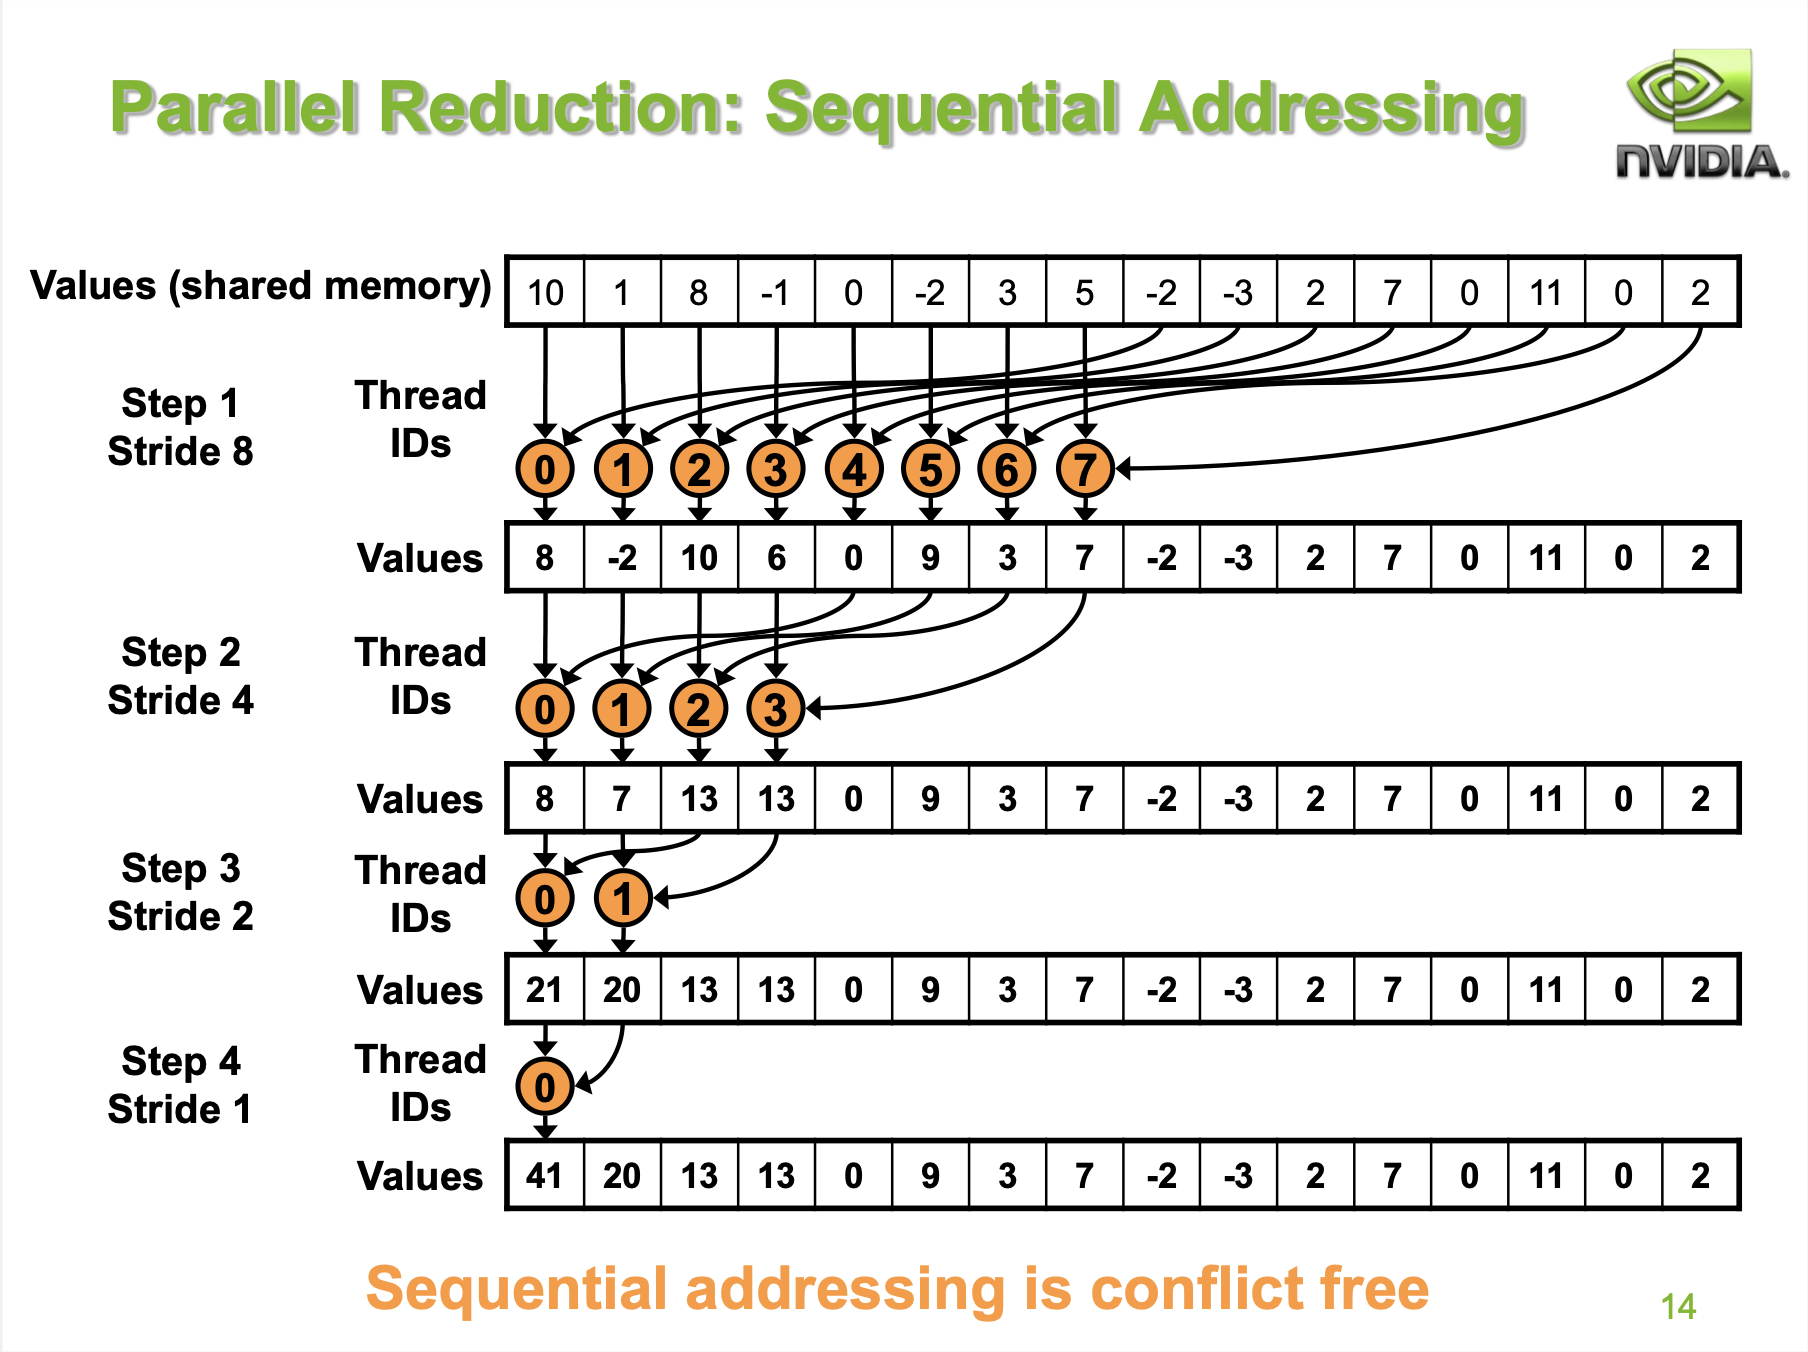
\includegraphics[width=12cm]{reduccion.png}
    \caption{Reducción paralela con direccionamiento secuencial para reducir un vector con la operación suma.
        Utilizamos esta misma estrategia en nuestro código.
        Extraído de \url{https://developer.download.nvidia.com/assets/cuda/files/reduction.pdf}.}
\end{figure}

\subsection{Análisis de la ejecución.}

Midiendo la utilización de los recursos de nuestra GPU descubrimos que la utilización del ancho de banda de memoria roza el
40\%, mientras que la capacidad de cómputo no llega al 60\%. Esto se debe a que aunque la ocupación de los \textit{Stream Processors}
alcanza su máximo efectivo aproximadamente el 90\% del tiempo los \textit{warps} están detenidos.
Analizando el código mediante la herramienta \textit{NVIDIA NSight Compute} descubrimos que la mayor parte del tiempo de ejecución
del kernel consiste en que el 30\% de los \textit{warps} acceden a memoria no residente en caché. El 55\% de las peticiones
de línea a caché de nivel uno fallaron y únicamente el 5\% de las peticiones de línea a caché de nivel dos tenían la línea preparada
para servirse.

Aun así, sin contar transferencias, nuestro algoritmo consigue aproximadamente una aceleración con respecto al algoritmo secuencial de CPU
de 68x. Si contamos transferencias encontramos con que este \textit{speedup} no alcanza el 2x.

Si el máximo número de entre todos los bloques lo encontramos en el \textit{host} con el algoritmo secuencial en vez de en el \textit{device}
obtenemos mejor aceleración.

Dado que la mayor parte del cuello de botella reside en las transferencias probamos a dividir los datos de entrada en distintos
bloques de forma que podamos, potencialmente, reducir la latencia. Para ello hacemos uso de \textit{streams}.
Descubrimos que, por alguna razón que no llegamos a investigar, la aceleración empeora hasta un 0.9x.

\subsection{Alternativas y trabajo futuro.}

Potencialmente nuestro \textit{kernel} podría mejorarse en gran medida cambiando el enfoque algorítmico y de transferencias de memoria.

Como alternativa podemos utilizar la librería \href{https://github.com/NVIDIA/thrust}{Thrust}, la cual junto a otras muchas utilidades
incluye un \textit{wrapper} para un algoritmo desarrollado por \textit{NVIDIA} para sus \textit{GPUs} para encontrar el máximo de un vector.

Si el código no fuese parte de otro algoritmo que se ejecutase en la GPU, sino que fuese un acelerador para la CPU, nos interesaría investigar
otras opciones como ciertas operaciones SIMD de la arquitectura x86 (o equivalentes según requiramos) como puede ser
\href{https://www.intel.com/content/www/us/en/docs/intrinsics-guide/index.html#text=_mm_cmplt_pd&ig_expand=1173}{\texttt{\_mm\_cmplt\_pd}.}
